\renewcommand\thetable{\arabic{chapter}-\arabic{table}}
%\renewcommand\thefigure{\arabic{chapter}-\arabic{figure}}
\chapter{校舍資訊與補強經費之關係模型}

校舍建築物的補強經費對於全國校舍的補強工作來說是非常重要的一個數值,和校舍的耐震能力並列因其直接表示了主管機關要讓該棟校舍符合耐震安全規範所需要的成本,教育部為了提升全國高中職及中小學校舍耐震能力,歷年來已經訂定及執行了各種評估與補強計劃。教育部將計畫委託國震中心執行,國震中心與教育部研擬商討後,再訂出執行計畫交由各縣市政府辦理。計劃的訂定需要資料的輔助,計劃的執行也需要定期的計劃報告以掌握計劃的執行進度與效力。全國校舍總數,經目前耐震資料庫中校舍普查作業已記錄之校舍數量統計共有~24930~棟,如果考慮尚未執行校舍普查作業之校舍,其實際校舍總數將更多。面對如此大量之校舍,進行總體或縣市為單位之經費估算,需耗費大量時間與人力進行估算與統計。且依照目前「高中職及國中小校舍結構耐震能力詳細評估作業規範」規定,主管機關須等到詳細評估之承攬廠商提送期末報告書,才能得知該校舍較精確之可能補強費用。由此可知,校舍補強經費的取得也是一個非常耗時且困難的流程,要提早在校舍進入詳細評估前就推估出校舍的補強經費,以往只能透過較為簡單的經驗公式推估,

目前主管機關在提撥補強校舍的耐震能力計畫的經費時,是每個年度依據需求估算,編列該年度的固定經費,根據教育部公布九十九年九月十六日修正之國中小校舍「補強工程」之經費支用範圍及參考單價計價方式,「補強工程」費用,包含了「直接補強工程費」、「合理之間接修復費」、「工程管理費」、「補強設計及監造費」等費用支出。依公告之估價方式將校舍分為「已完成補強設計」與「尚未完成補強設計」,歸類為「已完成補強設計」之校舍,其補強工程經費依補強設計審查通過或補強設計報告之金額,教育部原則將據 以如數核定補助經費。但其補強工程單價超出~$4000~\text{元}/m^2$~者,則應經補強設計期末審查或特別審查通過並附審查意見表,始能獲教育部如數核定補助經費;否則將依單價~$4000~\text{元}/m^2$~核定補助經費。歸類為「尚未完成補強設計」之校舍(凡未附補強設計審查意見表、未附補強設計報告重點摘要部分、或佐證資料不齊全者,皆屬尚未完成補強設計):其「補強工程」之參考單價計價方式依其總樓地板面積所屬級距範圍之不同,分別計算如表~\ref{tab:cost_result_table}~所示,其中「計價面積」係由「實際面積」以無條件進位為~2~的倍數之方式轉換而成;因此計價面積為~2~的倍數且為整數。例如:實際面積~$601~m^2$~,應轉換為計價面積~$602~m^2$。

\setlength{\tabcolsep}{1em}
\begin{table}[hbtp]
  \begin{center}
    \caption{補強工程參考單價之計價方式}
    \label{tab:cost_result_table}
    \begin{tabular}{l l}
      \hline
      建築物樓地板總面積 & 補強工程費用計算方式 \\
      \hline
      不足~$600~m^2$ & $\text{實際面積} \times 4000 \text{元}/m^2$ \\
      $600~m^2$~以上,不足~$3600~m^2$ & $\text{計價面積} \times (-0.5 \times \text{計價面積} + 4300) \text{元}/m^2$ \\
      $3600~m^2$~以上 & $\text{實際面積} \times 2500 \text{元}/m^2$ \\
      \hline
      \end{tabular}
  \end{center}
\end{table}

此一補強工程參考計價方式的主要依據是校舍的樓地板面積,但是實際影響補強經費的因素應該不只是校舍的樓地板面積,建築物的牆柱設計、施工品質、建造年代、不足的耐震能力等,對於補強的方式應該都有很大的影響,也間接的影響到補強經費,因此用此計價方式所得到的補強費用預估值是可靠度相對不足的數字,而此一預算編列的方式,是每年編列固定額度的預算,編列的年度預算難以在事後追加,使用可靠度不足的數字作為參考,會讓編列的預算與實際需求失準,而且每年固定的預算已經會讓每個年度能夠補強的校舍數量有所限制,對於不知何時會再發生的地震威脅,絕對是希望能夠儘快將最危險的校舍找出並做出對應處置,因此校舍耐震能力補強的經費編列和分配的影響就非常大,不過實際上在編列預算時,大部分校舍可能都還沒進行詳細評估、也還沒有建議的補強方案,因此只能透過參考資料和初步評估的資料來估算,如果可以在編列預算時,就能推估每間校舍的耐震能力、補強可能需要的經費,那麼主管機關在編列和分配預算的時候就可以非常有效率的來編列,因此本研究還試著找出校舍的基礎設計參數與其補強經費間的關係模型,透過這個模型,應該可以從校舍的初步評估資料得到一個可靠度交高的補強經費推估值。


\section{資料前處理}

本分析其構想為使用校舍評估階段初期之已調查資料來針對評估階段後期結果做預估。校舍耐震之補強工程經費須等到工程完成且承攬廠商提送竣工報告才能得知最後實際施工所花經費,因研究目標為達成前期預測之目的,所以需挑選補強施工以前之補強階段資料。校舍耐震評估與補強之流程如圖~\ref{fig:FLOW}~,可知進行補強施工之前尚須進行校舍普查、初步評估、詳細評估與補強設計,經了解各階段評估作業之內容與用途,校舍普查執行之人員為各大專院校之土木系學生 協助執行,且其所記錄之資料也較其他各階段為少,補強設計為補強施工之上一階段,根據「高中職及國中小校舍結構耐震能力補強設計作業 規範」規定,補強設計成果報告書中須編製工程預算書,因此即可於補強設計階段得知該補強工程之所需經費。為達研究之預測目的,本研究將採用初步評估與詳細評估(不含耐震補強方案)結果做為本探勘模型之選擇資料,並以典型校舍、鋼筋混凝土建築、單邊走廊且廊外無柱、無地下室、補強工程經費介於~100~至~1000~萬之間、初步評估與詳細評估均顯示為已送出之資料做為此模型資料選擇之條件篩選。

本模型採用初步評估與詳細評估(不含耐震補強方案)結果做為本探勘模型之選擇資料,並以典型校舍、鋼筋混凝土建築、單邊走廊且廊外無柱、無地下室、補強工程經費介於~100~至~1000~萬之間、初步評估與詳細評估均顯示為已送出之資料做為此模型資料選擇之條件篩選。模型經資料選擇與前處理之後建立資料集,下一步即是進行模型屬性之選擇,建立屬性集,本模型挑選之屬性集如下:

\begin{multicols}{2}
\begin{itemize}
\item 一樓樓地面積
\item 柱等效強度
\item 軟弱層顯著性
\item 裂縫鏽蝕滲水等程度
\item 短柱嚴重性
\item 調整因子
\item 二樓樓地板面積深
\item 二樓樓地板面積長
\item 樓層數
\item 二樓以上樓地板面積
\item 一樓教室柱根數
\item 一樓走廊外柱斷面積和
\item 非結構牆
\item X正向樑破壞
\item X正向柱破壞
\item X正向窗台柱破壞
\item X正向磚牆破壞
\item X正向性能點之屋頂最大位移
\item X正向性能點之等效基本週期
\item X正向性能點之基底剪力
\item 校舍耐震容量需求比
\item[]
\end{itemize}
\end{multicols}

以下為本預測模型屬性集內之屬性介紹與選擇說明:

\begin{description}
  \item[一樓樓地面積]
  依據教育部現行之補強工程計價公式如表~\ref{tab:cost_result_table}~,其經驗公式以樓地板面積為主要參數,而其可靠度雖然較差,但仍然是主管機關一個重要的參考數值,本分析所建立之模型為捕強工程經費與校舍設計參數間的關係,而校舍之樓地板面積也是一個非常重要的設計參數,可以代表校舍結構之規模,也隱含了校舍如果需要補強時,其規模大小之資訊在其中,因此本分析將此屬性拿來作為建立此關係模型之輸入屬性。
  \item[柱等效強度]
  柱之等效強度~$T_{AC}$~其計算公式為:

  \begin{equation}T_{AC} = (4+1.8NF) \times ClaAc+(2.4+1.08NF) \times CorAc+2.6 \times InsAc\end{equation} 

  其中~$NF$~為樓層數,~$ClaAc$~為一樓教室柱總斷面積,~$CorAc$~為一樓走廊外柱總斷面積,~$InsAc$~為一樓隔間柱總斷面積,其公式為根據三種類結構柱之單位斷面積極限剪力牆度計算公式~\cite{su2008master}~之加總,本分析將此屬性加入探勘模型之最初原因為該公式內有教室柱、走廊外柱與隔間柱於一樓的總斷面積,而此一數值和,並且因補強施工其所補強之面積愈大其所花錢就愈多。本分析經建立多組模型與各種屬性集之測試均發現該屬性對模型之預測結果有一定影響。
  \item[軟弱層顯著性]
  \cite{ncree03049}~若結構物之一樓因為使用性等考量,而使得二樓以上~RC~牆或磚牆於一樓中斷,致使一樓之極限層剪力強度與勁度降低,將造成地震力作用時變形集中,以致於韌性用盡,建築物就發生軟弱層破壞。故本表格依據牆體中斷的程度折減其對應之耐震能力,若~2/3~以上牆體中斷,則耐震能力折減為~0.8~倍;若~1/3~至~2/3~之牆體中斷,則耐震能力折減為~0.9~倍;若~1/3~以下之牆體中斷,則不折減其耐震能力。依此敘述得知軟弱層顯著性會影響結構物之耐震能力,結構物之耐震能力愈低,極可能所需補強之工程花費就愈高,因此本分析將此屬性納入本屬性集。
  \item[裂縫鏽蝕滲水等程度]
  \cite{ncree03049}~鋼筋混凝土構材若具有裂縫,代表混凝土品質不良或強度不足;保護層不足等因素使得鋼筋鏽蝕膨脹,鋼筋鏽蝕將會降低構材之強度,鋼筋鏽蝕膨脹亦會導致混凝土剝落,並加速鋼筋鏽蝕的程度,這些因素都會影響結構物的耐震安全,故以結構物整體之裂縫鏽蝕滲水等程度作為調整項目。若稍有裂縫鏽蝕滲水等情形,則耐震能力折減為~0.95~;若裂縫鏽蝕滲水等情形較為嚴重,則耐震能力折減為~0.9~;若無,則不折減其耐震能力。根據上述,建物若有裂縫鏽蝕滲水等情形會影響耐震能力,耐震能力愈差就有可能提升所需花費之工程經費,因此本分析將之納為輸入屬性。
  \item[短柱嚴重性]
  \cite{ncree03049}~一般老舊校舍之柱箍筋間距多為~20cm~至~30cm~左右,其剪力強度不高,且老舊校舍於設計時假設為純梁柱系統,並沒有考慮教室窗台及樓梯廁所等牆壁開氣窗所造成之短柱效應,然而這種短柱效應將會使得剪力容量不足之柱於地震時發生非預期之剪力破壞,導致結構韌性不足,若該校舍有過多之柱受到短柱效應之影響,將易造成校舍瞬間倒塌。故若校舍因窗台或氣窗造成短柱現象之柱根數達到全部柱根數之~50\%~以上,則耐震能力折減為~0.9~倍,若不足~50\%~則不予折減其耐震能力。值得注意的是,短柱嚴重性具有方向性,故評估時只需考慮評估方向之短柱比率是否超過一半即可,另一方向開窗等因素造成之短柱效應不需考慮。根據上述得知短柱現象為影響校舍耐震能力之原因之一,因此將之納入輸入屬性。
  \item[調整因子]
  \cite{ncree03049}~典型校舍初步評估表之六項調整因子調查項目,其功能為對初步評估耐震能力產生增減,包括:平面及立面對稱性、軟弱層顯著性、裂縫鏽蝕滲水等程度、變形程度、平面耐震性以及短柱嚴重性,定義~$q_1$~至~$q_6$~分別代表六項調整因子,其中軟弱層顯著性、裂縫鏽蝕滲水等程度和短柱嚴重性三項調整因子因對耐震能力之影響較為直接,所以也分別被納本分析之輸入屬性,而除此六項調整因子外,還有定義一整體調整因子~$Q$~為上述六項調整因子之乘積,整體調整因子代表所有調整因子對於耐震能力的折減或增加的幅度,其物理意義為校舍的現況對於校舍耐震能力影響的程度,對於校舍耐震能力來說也是很重要的一個參數,且經測試後證實該屬性對預測之正確性有提升,因此本分析也將其納入輸入屬性。
  \item[二樓樓地板面積深、深]
  依據教育部現行之補強工程計價公式如表~\ref{tab:cost_result_table}~,其公式以樓地板面積為主要參數,又面積之算法為長乘以寬(深),因此亦可將它視為影響校舍補強工程經費的因素之一。本分析所預測之目標為實際施工之工程總經費,與計價公式所估經費有直接關聯性,因此本分析將此二屬性拿來作為本預測模型之輸入屬性。
  \item[樓層數]
  樓層數愈高其總樓地板面積愈多,其總樓地板面積愈多,依補強工程計價公式如表~\ref{tab:cost_result_table}~。其工程經費預算就可能愈多,因此樓層數亦可視為影響工程經費之影響原因之一。
  \item[二樓以上樓地板面積]
  依據教育部現行之補強工程計價公式如表~\ref{tab:cost_result_table}~,其公式以樓地板面積為主要參數,本分析所預測之目標為實際施工之工程總經費,補強工程計價公式為經費預算之計算方式,估算出來之經費預算往往與實際施工所花經費不太一樣,預算可能高於實際施工也可能低於實際施工,但因為目標都是估算工程經費,因此本分析將此屬性拿來作為本預測模型之輸入屬性。
  \item[一樓教室柱根數]
  由校舍教室柱之數量可以間接得知校舍樓地板面積之大小或規模,且柱子的數量可以間接代表校舍乘載能力的大小,因此本分析將之視為影響工程經費之因素之一,經將此屬性納入探勘模型中測試後,也確實發現此屬性對預測之正確率有一定之提升。
  \item[一樓走廊外柱斷面積和]
  走廊外柱總斷面積愈大其意義可能有二:其一,斷面積愈大可能代表樓地板面積愈大,而根據補強經費估算的經驗公式,樓地板面積愈大其施工所需經費即可能愈高。其二,如果校舍樓地板面積大小一樣,但其廊外柱斷面積和比較大,代表其走廊外柱可能斷面積比較大,如果要進行擴柱補強工法,其工程所花經費就會比較高。綜合以上原因,本分析即嘗試將此屬性納入探勘模型中,並且經測試後效果不錯因此保留此屬性。
  \item[非結構牆]
  此屬性為記錄該校舍,有無非結構牆,並於分析時所建立模型是否有將該非結構牆模擬成其他等值桿件進入結構模型內。因有無非結構牆可能會影響校舍之耐震能力,而本分析之探勘目標包括了磚牆和~RC~牆是否破壞,,因此將之加入輸入變數。
  \item[X~正向樑破壞、X~正向柱破壞、X~正向窗台柱破壞、X~正向磚牆破壞]
  此四屬性為詳細評估資料表中之記錄欄位,記錄詳評後校舍可能優先破壞的構件以及其破壞的形式,此分析中根據實際詳細評估資料中的破壞趨勢選擇了包括~X~正向樑、~X~正向柱破壞、~X~正向窗台柱以及~X~正向磚牆四種構件的破壞模式,區分為無破壞、剪力破壞、撓剪破壞、撓曲破壞四種破壞形式,不同之破壞形式其需補強的方式會有所不統,其所需經費也不一樣,因此本分析將之列為本模型之輸入屬性。
  \item[X~正向性能點之屋頂最大位移]
  \cite{ncree08035}進行詳細評估時,若採用推垮分析,則該欄位則須依~X~及~Y~方向分別輸入屋頂最大位移值。本分析僅挑選採用推垮分析之校舍進行建模,因屋頂之最大位移為影響校舍耐震能力的因素之一,因此也將該屬性列入。
  \item[X~正向性能點之等效基本週期]
  \cite{ncree09015}基本週期為結構物等效單自由度系統的動力參數(性能目標地表加速度),此單自由度系統在性能目標地表加速度的設計地震作用下,其動力反應將是已設定的性能需求,因此基本週期亦是影響耐震能力評估結果的因素之一。
  \item[X~正向性能點之基底剪力]
  基底剪力為側推分析中計算容量曲線之重要參數之一,校舍之耐震能力可能影響補強之工程經費,因此本分析嘗試將此屬性放入本模型中進行測試,其結果對模型預測之正確率有提升,因此將它保留至屬性集之中。
  \item[校舍耐震容量需求比]
  \cite{ncree09026}校舍建築物進行耐震初步評估後,得到一耐震指標分數~$Is$~,此耐震指標可作為是否需進入下一階段評估工作的參數,同樣地,經由專業人員完成詳細評估後,得到建築物長短向最大可抵抗之地表加速度,除以該校舍~475~年回歸期設計地表加速度,稱之耐震容量需求比(Capacity Demand Ratio,CDR),此數值若小於~1~時,則判定該棟建築須進行補強;反之,該棟建築耐震能力暫無疑慮,但仍須定期檢視。根據上述得知~$CDR$~可視為該校舍之耐震能力與正常安全值之距離,如果數值小於~1~且離~1~愈遠,代表需替該校舍提升的耐震能力愈多,所需花的經費就愈多,因此亦可視為影響補強工經費之因子。
\end{description}

\section{資料探勘}

本分析採用類神經網路與~CHAID~決策樹進行資料探勘之建模,選擇此二種探勘方法,主因為本分析之預測目標,總工程經費為連續數值,最適合使用的探勘演算法為迴歸演算法,因此挑選其中應用範圍最廣的類神經網路做為基準,另外屬於決策樹方法分支之~CHAID~決策樹經初步測試應用於本分析之預測目標,其表現不錯,因此本分析以此二種探勘方法,使用前處理完之~235~筆資料,將整體資料採亂數選取方式分為~85\%~為訓練區與~15\%~為測試區,類神經網路之設定為使用~Multilayer Perceptron~之網路形式,並讓~SPSS Clemitine~自動計算隱藏層數量及各層節點數,訓練~15~分鐘,然後挑出表現最的一組神經網路。CHAID~決策樹之模型設定為:最大決策樹深度為五層,停止條件為決策節點之資料筆數為總數之~1\%,SPSS Clemitine~之節點架構如圖~\ref{fig:cob-flow}~所示,模型之訓練結果如表~\ref{tab:cost_result}。

\begin{figure}[hbtp]
  \begin{center}
    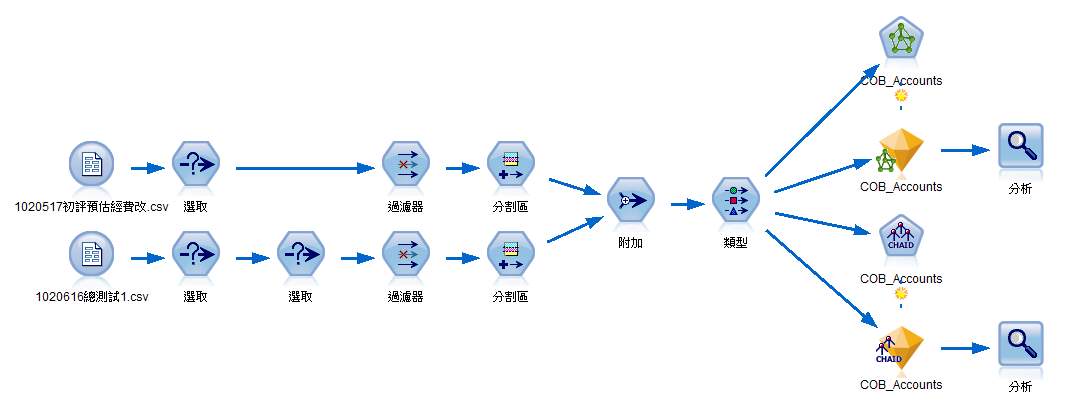
\includegraphics[width=1.0\textwidth]{figures/cob-flow.png}
    \caption{補強經費模型探勘流程} 
    \label{fig:cob-flow}
  \end{center}
\end{figure}

%先行根據既有知識挑選資料集內之欄位並配合使用試誤法直到找出最佳做為探勘模型之屬性集,做為模型訓練方法。

%最後再挑一組結果較好之模型與屬性集保留。本模型之訓練結果如表~\ref{tab:cost_result},因本模型之整體資料較少,其結果之線性相關程度目前呈現比較低。

\begin{table}[hbtp]
  \begin{center}
    \caption{Result of the Retrofit Cost Model}
    \label{tab:cost_result}
    \large
    \begin{tabular}{l c c c c}
      \hline
       & \multicolumn{2}{c}{ANNs} & \multicolumn{2}{c}{CHAID} \\
       & Training & Testing & Training & Testing \\
      \hline
	   R & 0.812 & 0.949 & 0.718 & 0.874 \\
      \hline
      \end{tabular}
  \end{center}
\end{table}

\section{結果}

本資料探勘分析結果得到兩個可以從校舍基本設計資料得到其補強所需經費之關係模型,分別為使用類神經網路及 CHAID 決策樹所探勘得到,表~\ref{tab:cost_result_2}~為此兩二模型不分測試訓練集之~$R^2$~與~MAPE~。CHAID 模型之推估值與實際值之比較如圖~\ref{fig:cob-chaid-vs}~所示,而類神經網路模型之推估值與實際值之比較如圖~\ref{fig:cob-ann-vs}~所示。兩者比較可以發現~CHAID~因為其知識形式為決策樹之特性,所得到的推估值只有數種可能性,造成其~MAPE~較高,但是其在圖~\ref{fig:cob-chaid-vs}~上所呈現之線性關係較好,表示此模型仍保有正確之關係於模型之中,而根據圖~\ref{fig:cob-chaid-vs}~可以發現其誤差方向之分佈尚且平均,計算~235~棟校舍之平均誤差量僅為~11066~元,類神經網路模型之平均誤差量則為~33512~元,顯示此一模型尚可以用在大量校舍之整體補強預算評估上,然而如果要推估單棟校舍之補強經費,則建議使用類神經網路探勘所得到之模型,類神經網路所產生模型之線性關係較~CHAID~產出之模型來的差,根據圖~\ref{fig:cob-ann-vs}~可以發現其數據較為集中,只是其趨勢與~$x = y$~之目標趨勢方向不同,表示此模型有確實的呈現校舍設計參數與其補強費用間的關係趨勢,然而線性關係表現較差,顯示仍然有些影響補強經費的因素尚未被找出。

\begin{table}[hbtp]
  \begin{center}
    \caption{Result of the Retrofit Cost Model without Testing}
    \label{tab:cost_result_2}
    \large
    \begin{tabular}{l c c}
      \hline
       & ANNs & CHAID \\
      \hline
     $R^2$ & 0.69 & 0.54 \\
     MAPE & 26.43\% & 28.91\% \\
      \hline
      \end{tabular}
  \end{center}
\end{table}


\begin{figure}[hbtp]
  \begin{center}
    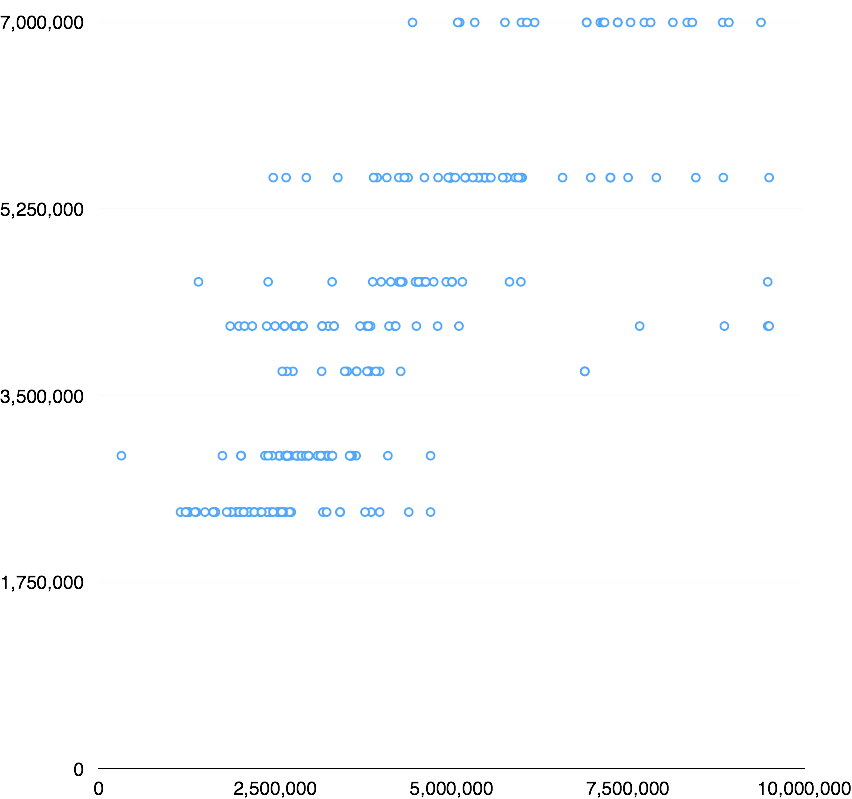
\includegraphics[width=0.6\textwidth]{figures/cob-chaid-vs.png}
    \caption{補強經費實際值 vs CHAID 模型預估值} 
    \label{fig:cob-chaid-vs}
  \end{center}
\end{figure}


\begin{figure}[hbtp]
  \begin{center}
    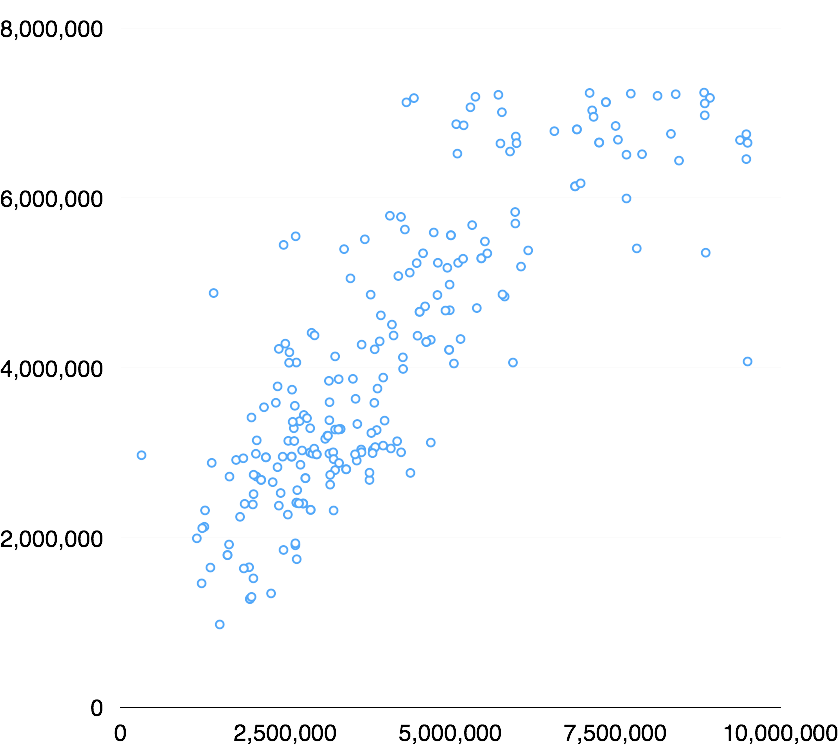
\includegraphics[width=0.6\textwidth]{figures/cob-ann-vs.png}
    \caption{補強經費實際值 vs ANN 模型預估值} 
    \label{fig:cob-ann-vs}
  \end{center}
\end{figure}


%雖然相較於~CHAID~決策樹,類神經網路的表現較差,

%本分析用來判斷模型優劣的指標為~$R^2$~和~MAPE~,~MAPE~用來表示模型預測值的平均誤差,為一百分比索引值,數值越小表示模型品質越好,使用此一指標的主因在於可以用來評估此迴歸模型所估算之補強經費,其誤差可能造成之經費差距有多少,對於主管機關來說也是一個非常重要的參考依據,根據表~\ref{tab:cost_result}~,類神經網路和~CHAID~決策樹的表現均很接近,且其測試集的表現顯示此二模型均有其可靠性,最後選擇使用類神經網路作為最後挑選的模型,不分訓練測試集重新訓練建立關係模型,結果其~MAPE~為~31.8\%~,~$R^2$(相關係數)為~0.9004~,可以發現~$R^2$~的表現很好,表示此模型有確實的呈現校舍設計參數與其補強費用間的關係趨勢,然而~MAPE~表現較差,顯示仍然有些影響補強經費的因素尚未被找出。






